% Chapter 1

\chapter{Implementation} % Main chapter title

\label{Chapter3} % For referencing the chapter elsewhere, use \ref{Chapter1} 

%----------------------------------------------------------------------------------------

% % Define some commands to keep the formatting separated from the content 
% \newcommand{\keyword}[1]{\textbf{#1}}
% \newcommand{\tabhead}[1]{\textbf{#1}}
% \newcommand{\code}[1]{\texttt{#1}}
% \newcommand{\file}[1]{\texttt{\bfseries#1}}
% \newcommand{\option}[1]{\texttt{\itshape#1}}

%----------------------------------------------------------------------------------------

This project followed a non-standard approach to software development which incorporated aspects of various software engineering standards. The general approach to implementation followed the design philosophy of dependency injection.

The scope of this project involved conceptualising and designing a software system as well as implementing a working prototype of said software for a specific virtualisation platform. Three high powered computer servers were used to build up the hardware environment. In this instance, OpenStack was chosen as the appropriate provider environment. OpenStack is industry-ready software that is currently being utilised for cloud projects in academia around South Africa, such as with the Inter-University Institute for Data Intensive Astronomy (IDIA) and South African Data Intensive Research Cloud (SADIRC), previously known as the African Research Cloud (ARC).

\section{Backend}

\subsection{Hardware}

Decommissioned hardware from the Physical Science department was donated in order to be used for e-research efforts at the University of the Western Cape. Some of the hardware donated was utilised for this project. Table \ref{tab:hardware} details the hardware specification.

\begin{table}[ht!]
\caption[OpenStack Server Hardware Specification Table]{Hardware specification of the servers used to host OpenStack.}
\centering
\label{tab:hardware}
\resizebox{\textwidth}{!}{%
\begin{tabular}{p{0.15\linewidth}p{0.2\linewidth}p{0.2\linewidth}p{0.15\linewidth}p{0.15\linewidth}p{0.2\linewidth}}
\toprule
Description    & Physical Device           & CPU                                  & Memory                           & Storage            & Network                                                                                                     \\ \midrule
Controller & Supermicro CSE-512F-350B  & AMD Opteron 4334 - 6 cores @ 3.1GHz  & 64GB Samsung DDR3 @ 1600MHz ECC  & 223.6GB RAID1 SSDs & \begin{tabular}[c]{@{}p{1\linewidth}@{}}x4 Intel I350 Gigabit Network Connection;\\ x2 10-Gigabit X540-AT2\end{tabular}  \\
Compute             & Supermicro AS-2042G-72RF4 & AMD Opteron 6348 - 48 cores @ 2.8GHz & 256GB Samsung DDR3 @ 1600MHz ECC & 13.7TA RAID5 HDDs  & \begin{tabular}[c]{@{}p{1\linewidth}@{}}x4 Intel I350 Gigabit Network Connection;\\ x2 10-Gigabit X540-AT2\end{tabular} \\
Storage             & Supermicro AS-2024G-72RF4 & AMD Opteron 6348 - 48 cores @ 2.8GHz & 256GB Samsung DDR3 @ 1600MHz ECC & 13.7TA RAID5 HDDs  & \begin{tabular}[c]{@{}p{1\linewidth}@{}}x4 Intel I350 Gigabit Network Connection;\\ x2 10-Gigabit X540-AT2\end{tabular}  \\ \bottomrule
\end{tabular}%
}
\end{table}

Other than the server hardware, two network switches were utilised. One switch was used for internal university network access as well as management and operated at 10 Gbps. The other switch provided access externally to the internet directly.

\subsection{OpenStack}

The following section will detail the various components of OpenStack that were used in the implementation of the project, as well as the components of Nikeza and how they interact with them.

OpenStack is a highly modular open source IaaS platform that can be self-hosted at any institution. There are various components in use for this project to achieve the set goals.

Figure \ref{fig:network_layout} describes the hardware layout that hosts the OpenStack installation. The various services that make up the cloud environment are distributed among them. Each of the servers on which the OpenStack installation is placed was loaded with Ubuntu Server 16.04.2 as their operating systems. OpenStack Newton was chosen as the release for the project, due to it being the newest at the initiation time.

\begin{figure}[ht!]
\centering
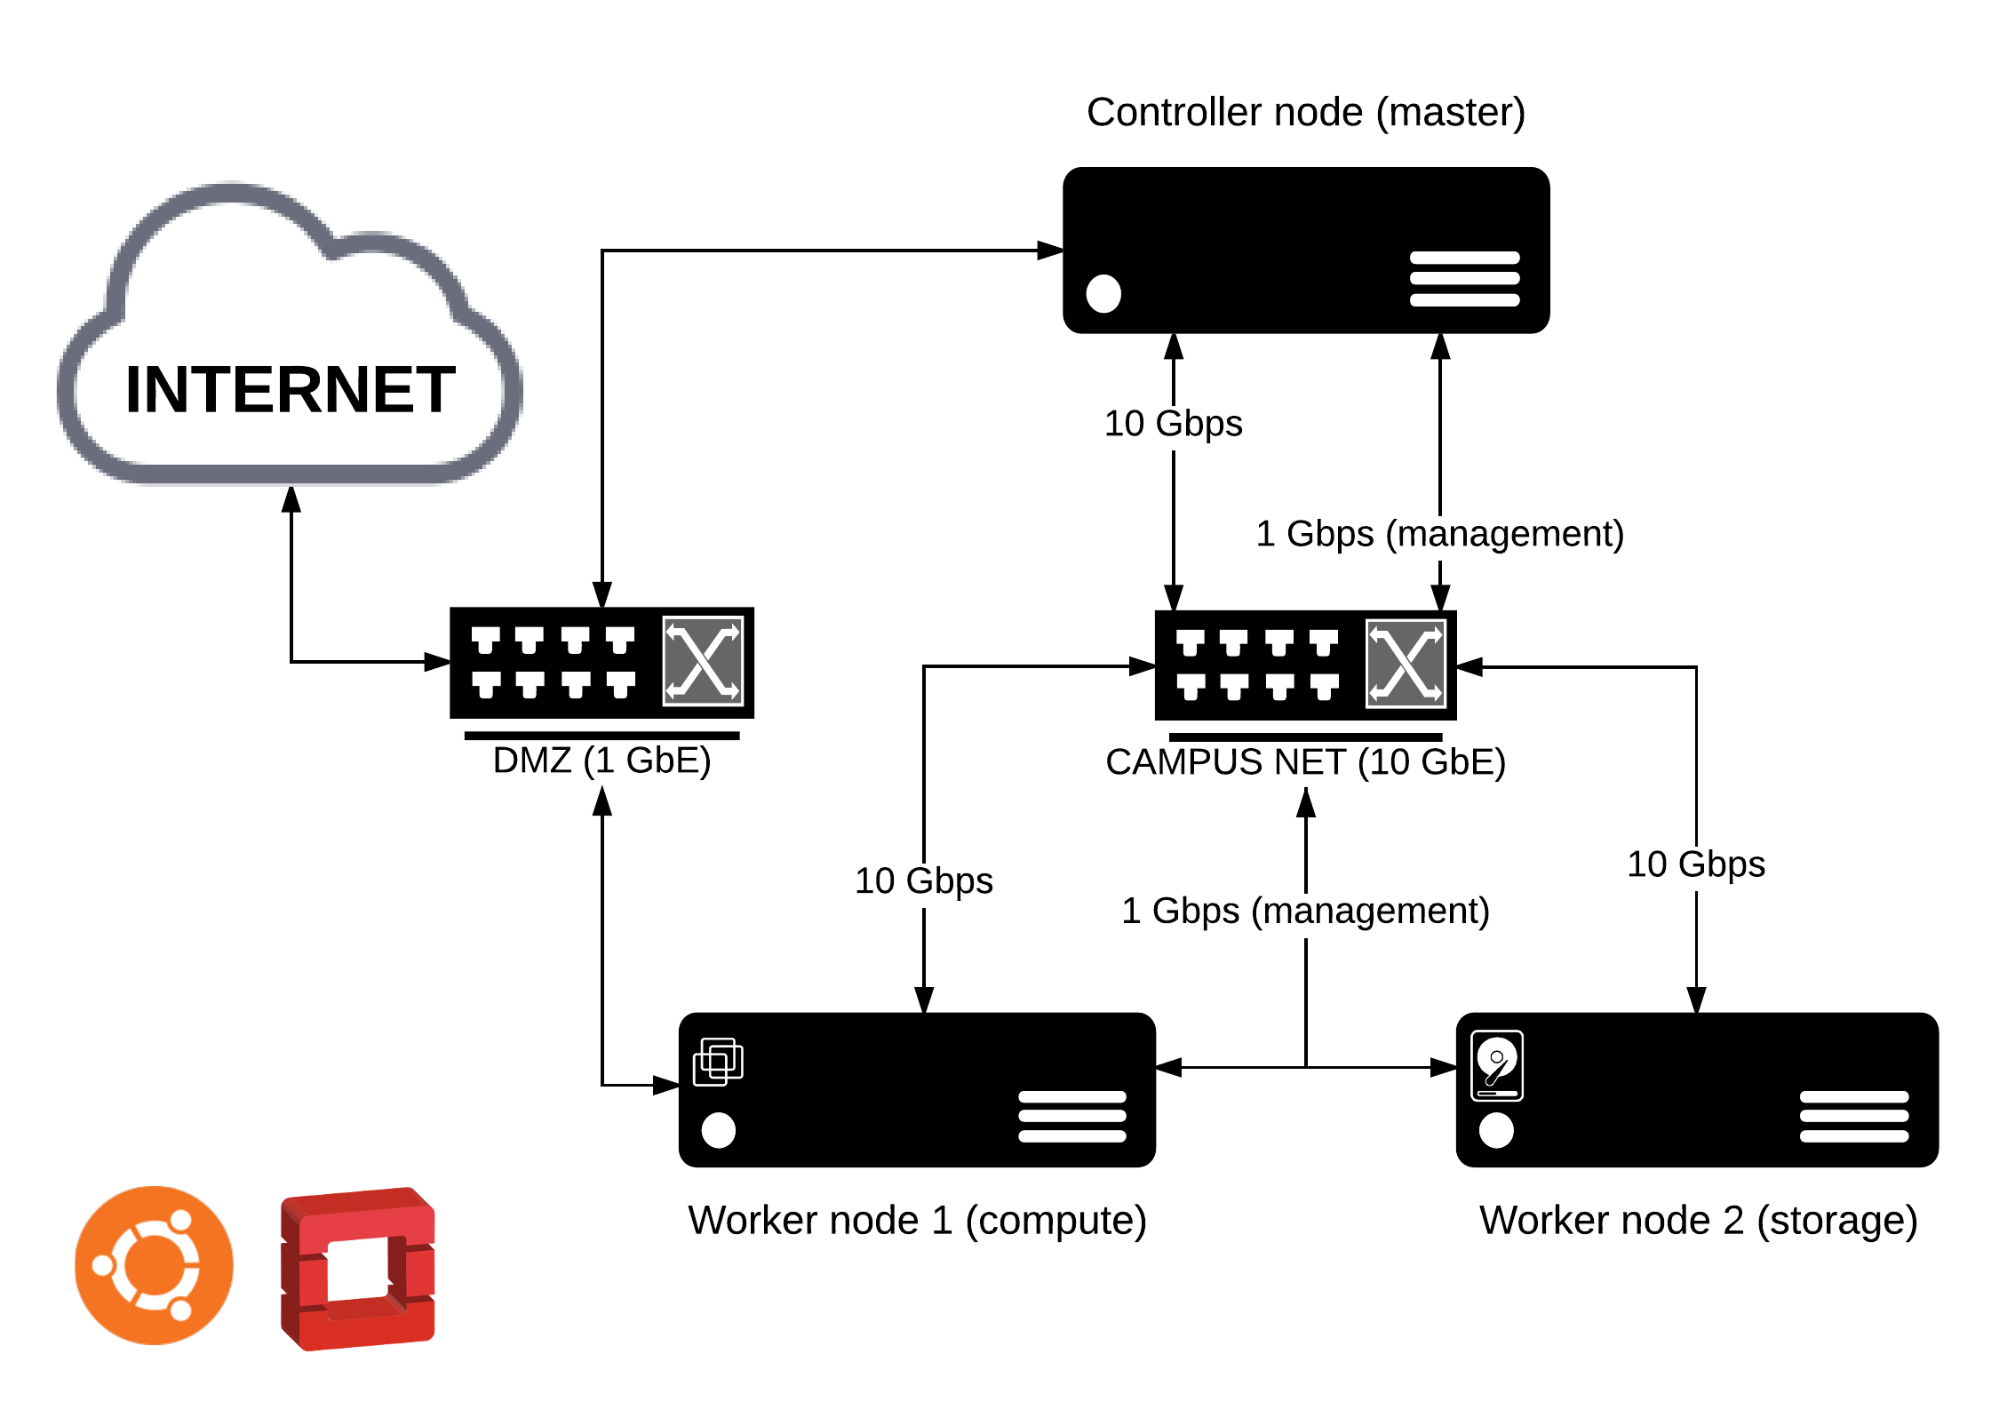
\includegraphics[width=\textwidth]{Figures/3_hardware_layout_network.png}
\decoRule
\caption[OpenStack Hardware and Network Layout]{The university-supplied internet was connected to the OpenStack controller and compute node directly. OpenStack services communicated via a 10 Gbps network and the management network was run over a more typical 1 Gbps private network.}
\label{fig:network_layout}
\end{figure}

The controller node acted as the orchestrator. Instructions are delivered to it through Nikeza and it creates virtual compute instances (virtual machines) on the first worker node while utilising storage and data that is located on the second worker node.

Each server was interconnected with 10 Gbps networking for OpenStack to communicate to all its respective services with low latency. All of the nodes were then connected to the internal network of the University of the Western Cape (UWC) through 1 Gbps interconnects to be able to interact with it and create virtual machines that use IP addresses from the UWC pool, so as to not create unnecessary security vulnerabilities by exposing the virtual machines directly to the internet. The controller and the compute worker node were connected directly to the outside internet through the DMZ on a 1 Gbps connection, in order to configure OpenStack services without IP security and port filtering rules that are in place with the standard university network.

\subsubsection{Controller Node}

The controller node aggregates and instructs services that are on other nodes. Various OpenStack services are run on this machine in order to achieve this\footnote{Installation instructions used for the OpenStack services were provided by the official documentation found at \url{https://docs.openstack.org/newton/install-guide-ubuntu/}}. The services that were on the controller node are described in Table \ref{tab:openstack_controller_services}.

\begin{longtable}[c]{@{}p{0.12\linewidth}p{0.12\linewidth}p{0.1\linewidth}p{0.55\linewidth}@{}}
\caption[OpenStack Controller Node Service List]{OpenStack services on the Controller node.}
\label{tab:openstack_controller_services}\\
\toprule
Service  & Type          & Version & Description                                                                                                                                                                                                                                                                                             \\* \midrule
\endhead
%
\bottomrule
\endfoot
%
\endlastfoot
%
Keystone & Identity      & 10.0.1  & Keystone provides an identity service to OpenStack. This provides authentication, authorisation, and cataloging of services. User accounts and roles can be created to restrict access where appropriate. Other OpenStack services also utilise it to understand which context they need to operate in. \\
Glance   & Image         & 9.1.2   & Virtual instances that are spawned on the compute node (worker node 1) need to have operating systems installed to them. Glance provides an imaging service that can store bootable images and provide them to running virtual instances on creation.                                                   \\
Nova     & Compute       & 14.0.4  & Various modules make up Nova. The controller node has Nova management services installed in order to orchestrate and manage and compute nodes that are in the OpenStack deployment.                                                                                                                     \\
Neutron  & Network       & 9.2.0   & Neutron provides OpenStack with a service that can manage virtual networks. Virtual network adapters and routes can be created to manage access to virtual instances. It provides a plugin system that allows support for various different external network configurations.                           \\
Horizon  & Dashboard     & 10.0.2  & The dashboard is an easy to use web interface to manage OpenStack as an administrator or a user.                                                                                                                                                                                                        \\
Cinder   & Block Storage & 9.1.2   & Virtual instances require disk storage to place files for operating system deployment and operation. Cinder provides block storage from any nodes running the necessary services to the virtual instances.                                                                                              \\
Swift    & Object Store  & 10.1    & Swift is an object store service that works within the OpenStack context. It is useful for storing large unstructured data. A proxy service for managing requests for data and user authentication to the storage nodes.                                                                                \\* \bottomrule
\end{longtable}

\subsubsection{Worker Node 1 (Compute)}

The first worker node was designated as the server that will handle the execution of virtual and containerised environments. This server will make use of the services available through the second worker node as well as the controller node and it is managed through the controller node. The services that are on the first worker node are described in Table \ref{tab:openstack_worker1_services}.

% Please add the following required packages to your document preamble:
% \usepackage{booktabs}
% \usepackage{longtable}
% Note: It may be necessary to compile the document several times to get a multi-page table to line up properly
\begin{longtable}[c]{@{}p{0.12\linewidth}p{0.12\linewidth}p{0.1\linewidth}p{0.55\linewidth}@{}}
\caption[OpenStack Compute Node Service List]{OpenStack services running on the Compute node.}
\label{tab:openstack_worker1_services}\\
\toprule
Service & Type    & Version & Description                                                                                                                                                                                                               
 \\* \midrule
\endhead
%
Nova    & Compute & 14.0.4  & The Nova services that runs on the compute node is comprised of a group of modules that allow for the execution of virtual machines under a pre-decided hypervisor. Since the hardware this project runs on supports hardware acceleration, the KVM hypervisor was used.                                                                                           \\
Neutron & Network & 9.2.0   & The Neutron services that run on the compute node allow for connectivity and routing from and to virtual machine instances. \\*
\bottomrule
\end{longtable}

\subsubsection{Worker Node 2 (Storage)}

The second worker node was dedicated as the storage node. This node provides block storage to all virtual instances created by the compute node, as well as the object store services which allow the storage and retrieval of data. The services running on the second worker node are described in Table \ref{tab:openstack_worker2_services}.

\begin{longtable}[c]{@{}p{0.12\linewidth}p{0.12\linewidth}p{0.1\linewidth}p{0.55\linewidth}@{}}
\caption[OpenStack Storage Node Service List]{OpenStack services running on the Storage node.}
\label{tab:openstack_worker2_services}\\
\toprule
Service & Type          & Version & Description                                                                                                                                                                                                              \\* \midrule
\endhead
%
Cinder  & Block Storage & 9.1.2   & The Cinder service on the storage node makes use of the LVM driver in order to provision physical storage that exists on it for virtual machine instances to use via iSCSI transport.               \\
Swift   & Object Store  & 10.1    & The Neutron services that run on the compute node allow for connectivity and routing from and to virtual machine instances. \\* \bottomrule
\end{longtable}

\subsection{Software}

The Python Flask micro-framework was used to rapidly create and deploy the various stages of this application.

\subsubsection{Project Breakdown}

Scheme \ref{sch:dir_tree} provides a full overview of the layout of the project on the filesystem. Where applicable, an asterisk was used in order to demonstrate that there are files in a directory that are unimportant to the operation of the software program, such as layout files.

\begin{scheme}[ht!]
% \renewcommand*\DTstylecomment{\rmfamily\color{green}\textsc}
% \renewcommand*\DTstyle{\ttfamily\textcolor{red}}
\centering
\scalebox{0.7}{\begin{minipage}{\textwidth}
\dirtree{%
.1 /.
.2 Nikeza.py\DTcomment{The main Flask application definition.}.
.2 operations\DTcomment{Directory for operational scripts.}.
.3 cloud-init.yml\DTcomment{Common cloud-init commands for VMs.}.
.2 operations.py\DTcomment{The bulk of the operational functions for working.}.
.2 parser.py\DTcomment{Parsing configuration file.}.
.2 plugins\DTcomment{Directory for plugin system.}.
.3 backend\DTcomment{Backend cloud-engine plugins.}.
.4 openstack\_bash.py\DTcomment{Plugin file to operate OpenStack with Bash.}.
.3 storage\DTcomment{Storage backend plugin.}.
.4 swift.py\DTcomment{Plugin file to operate with Swift storage.}.
.2 static\DTcomment{Directory for static media used to render frontend.}.
.3 custom.js\DTcomment{Custom JavaScript for Nikeza frontend.}.
.3 fonts\DTcomment{Fonts for Nikeza frontend.}.
.4 *\DTcomment{Various fonts.}.
.3 images\DTcomment{Images for Nikeza frontend.}.
.4 *\DTcomment{Various images.}.
.3 jstree\DTcomment{jsTree plugin for tree-view data selection.\footnotemark[\the\numexpr\value{footnote}+1]}.
.4 *\DTcomment{Various plugin files.}.
.3 materialize\DTcomment{A CSS and Javascript framework for web.\footnotemark[\the\numexpr\value{footnote}+2]}.
.4 *\DTcomment{Various framework files.}.
.3 style.css\DTcomment{Custom CSS stylesheet for frontend.}.
.2 templates\DTcomment{Directory for frontend templates.}.
.3 index.html\DTcomment{Main page for frontend.}.
.3 main.html\DTcomment{Common code shared between template files.}.
.3 new.html\DTcomment{Page for creating new job.}.
.3 queue.html\DTcomment{Page to view existing jobs.}.
.2 vars.conf\DTcomment{Variables for Nikeza runtime.}.
}
\par\null\par
*= Various unimportant files
\end{minipage}
}
\caption[Directory Tree]{Project filesystem tree hierarchy.}
\label{sch:dir_tree}
\end{scheme}
\refstepcounter{footnote}\footnotetext{jsTree by Ivan Bozhanov, \url{http://vakata.com}}
\refstepcounter{footnote}\footnotetext{MaterializeCSS framework by Materialize, \url{http://materializecss.com}}


% \begin{figure}[ht!]
% \centering
% 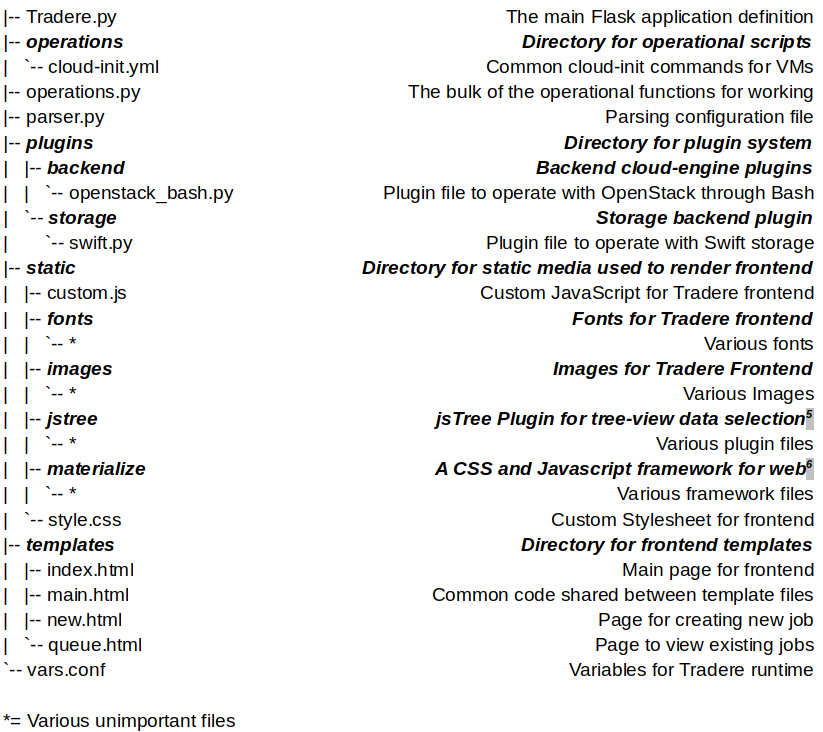
\includegraphics[width=\textwidth]{Figures/3_dir_tree.png}
% \decoRule
% \caption[Directory Tree]{Project filesystem tree hierarchy.}
% \label{fig:dir_tree}
% \end{figure}

\subsubsection{Module Dependencies}

Figure \ref{fig:module_deps} gives a visual representation of the interaction of modules and dependencies between them in the project.

\begin{figure}[ht!]
\centering
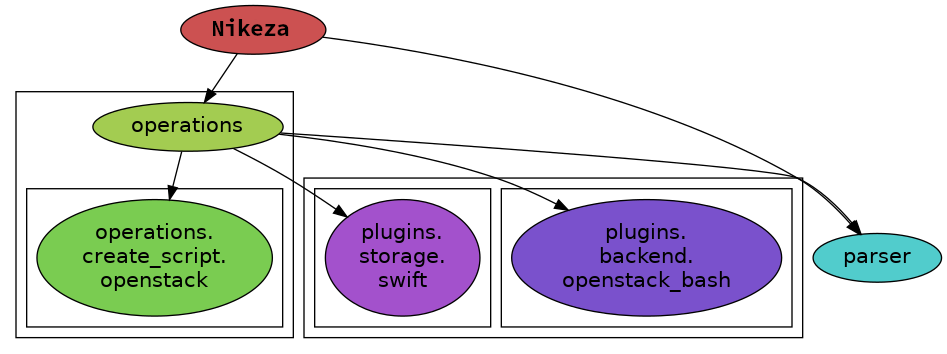
\includegraphics[width=\textwidth]{Figures/3_module_deps_new.png}
\decoRule
\caption[Nikeza Software Module Dependencies]{This figure shows the module dependencies diagram in the context of the Nikeza software.}
\label{fig:module_deps}
\end{figure}

Plugins are used with the Nikeza system in order to allow functionality with different backend cloud systems and storage services. The way this is achieved is to have a file called "vars.conf" which contains all the configuration variables for runtime. The configuration parameters are detailed in scheme \ref{sch:system_params}.

\begin{scheme}[ht!]
\makebox[\textwidth]{\fbox{%
\centering
\begin{minipage}{0.975\textwidth}
\textbf{[GENERAL]\dotfill {\small Contains variables for general configuration.}}\\
sysname=SANBI\dotfill    {\small The name of the organisation running the software}.
\par\null\par
\textbf{[BACKEND]\dotfill    {\small Contains variables for the cloud system.}}\\
platform\_name=OpenStack\dotfill    {\small The name of the backend system.} \\
platform\_file=openstack\_bash.py\dotfill    {\small The name of the plugin file for the system.} \\
platform\_image=openstack-icon.png\dotfill    {\small The name of an icon file for the system.} \\
\par\null\par
\textbf{[SYSTEM]\dotfill    {\small Contains variables for the storage system.}}\\
storage\_backend=swift.py\dotfill   {\small The name of the plugin file for the storage system.}\\
storage\_url=http://controller.cluster\dotfill    {\small The URL to access the storage with.}\\
storage\_port=8080\dotfill    {\small The port to accompany the URL.}\\
\par\null\par
\textbf{[OPERATIONS]\dotfill    {\small Contains variables for virtual machine operation.}}\\
ops\_cloudinit=cloud-init.yml\dotfill    {\small The name of the cloud-init bootstrap script.}\\
ops\_postscript=post-instance.sh\dotfill    {\small The name of the script which executes in VM.}\\
\end{minipage}
}}
\caption[System Parameters]{Global configuration file details.}
\label{sch:system_params}
\end{scheme}

The plugin files themselves are defined with a common set of classes and methods so that the operational script can successfully create instances and call methods as expected. This applies to both the cloud backend plugin and the storage system plugin.

\subsubsection{Web Rendering}

The main application file, "Nikeza.py", is used to start the Flask server, handle connections and sessions, and render the web pages. When a user navigates to one of the endpoints defined by "Nikeza.py", logic is applied to that connection and the appropriate web template is built and served to the user. This script makes use of the "operations.py" script, which handles all the backend service and platform interaction.

\subsubsection{Main Operations}

The script named "operations.py" contains all of the operations that are required for interacting with the backend environment and storage. The specifics of the interactions are detailed in the following two sections.

This file will parse the "vars.conf" file and collect all the information necessary to the application's run. It then pulls in the cloud and storage environment files as dependencies and uses their methods in order to provide the application with responses from the respective environments.

\subsubsection{Cloud Backend}

The "operations.py" script has a variable named "plugin". This variable is used to load the backend plugin file indicated by the "platform\_file" configuration line in the "vars.conf" file. This contains all the interaction commands and definitions for the cloud or appropriate backend environment that is in place. 

The file specified by "platform\_file" contains a set of common methods that can be called by the "operations.py" file. That is to say, the file specified by "platform\_file" behaves as the skeleton, or abstraction, of the backend for Nikeza. The common methods have to have a constant naming scheme between any files written for "platform\_file". These methods will have specific logic for starting virtual environments, listing running virtual machines, stopping virtual machines and retrieving IP addresses of virtual machines.

\subsubsection{Storage Backend}

Similarly to how the cloud backend is handled, the "operations.py" script contains a variable named "storage", which is used to load the storage plugin specified by the "storage\_backend" line of "vars.conf". This contains all the interaction commands and definitions for the object storage environment being used.

As with the cloud backend, the file specified by "storage\_backend" contains a set of common methods for interacting with the storage environment. This also abstracts the storage environment and allows a specific environment to be swapped out, as long as the new file is also using the same names. The methods in this file include getting the overview of the object storage contents, traversal of directories on the object store, getting object IDs and getting URLs that link to the objects in order to pull them into the virtual machines.

\subsubsection{Workflow Language}

The Common Workflow Language (CWL) specification was chosen to be used in the proof-of-concept system. This is a simple-to-learn and write language specification for researchers to wrap their pipeline into a single flowing set of reproducible instructions. The workflow language or tool chosen for the project is not critically important, as ideally many different types would be supported. For the purposes of this project, CWL is appropriate to test with due to it having various sample workflows to test.

CWL affords various executors, which are tools that parse and execute the specification. These executors offer all sorts of different functionality and targets, such as the Toil executor which can execute CWL workflows against cloud environments such as Amazon AWS. The CWL group also provides a reference executor which implements the basic functionality that a CWL executor should possess. This was deemed to be the simplest tool to use to answer the project aims posed in Chapter \ref{Chapter1}.

\subsubsection{Container System}

Docker was chosen as the container engine due to its large selection of container images available on its public repository, Docker Hub/Store, as well as it having the largest community involvement and support. The only other container engine that was considered was Singularity, due to its more research-driven focus. Singularity also allows containers to execute in a non-root environment, meaning potentially fewer complications in terms of security. 

However, due to the fact that a virtual machine is created for the researcher's execution environment and only the data that the researcher will use with the containerised tools is pulled into the said virtual machine, it was decided that Docker will be suitable. Any security risk that is presented by Docker is negated by the extra hypervisor security layer, as well as the fact that the potential attacker would already have access to the data pulled into the virtual environment even if it was through Singularity. The project was already well underway before Singularity was noticed.

There are various container orchestration systems, such as Docker Swarm\footnote{\url{https://docs.docker.com/engine/swarm/}}, Kubernetes\footnote{\url{https://kubernetes.io/}}, Red Hat OpenShift\footnote{\url{https://www.openshift.com/}} and Apache Mesos\footnote{\url{https://mesos.apache.org/}}. All of these serve to provide scheduling for multiple container instances to work together, have complex networking and communicate with shared storage together, which in turn allows them to perform more complex workloads. Originally, OpenStack's "Magnum" API extension\footnote{\url{https://wiki.openstack.org/wiki/Magnum}} was considered to be used as the core for Nikeza on OpenStack. This would have provided Nikeza native use of either Docker Swarm or Kubernetes on top of OpenStack, but it proved to be too time-consuming to implement due to the immaturity of the "Magnum" project at the time.

\section{Frontend}

The frontend part of the system is the section that the end user, or researcher, deals with directly when engaging with the project. This is the visual representation that is exposed to them. This is provided through a website that they interact with.

With reference to the above project breakdown scheme \ref{sch:dir_tree}, the "static" and "template" directories belong to the frontend part of the system. The "template" directory contains the template HTML documents that are rendered through the backend when the user requests an appropriate page. The "static" directory contains all the assets used to provide features and visuals to the user.

\section{Tools}

I would like to acknowledge that the following tools were utilised in order to complete the software project:

\begin{itemize}
    \item JetBrains PyCharm\footnote{\url{https://www.jetbrains.com/pycharm/}} - A Python Integrated Development Environment (IDE).
    \item GitHub Atom\footnote{\url{https://atom.io/}} - An Electron based hackable text editor.
    \item GitHub\footnote{\url{https://github.com/}} - A free online Git repository for source control.
    \item Pydepgraph\footnote{\url{https://github.com/stefano-maggiolo/pydepgraph}} - A tool to generate module dependency graphs for Python scripts.
\end{itemize}